%%----------------------------------------------------------------------------
%% Onderzoekstechnieken: De centrale limietstelling
%%----------------------------------------------------------------------------

\documentclass[aspectratio=169]{beamer}

%==============================================================================
% Aanloop
%==============================================================================

%---------- Vormgeving --------------------------------------------------------

\usetheme{hogent}

\usecolortheme{hgwhite} % witte achtergrond, zwarte tekst

\usepackage{graphicx,multicol}
\usepackage{comment,enumerate,hyperref}
\usepackage{amsmath,amsfonts,amssymb}
\usepackage[dutch]{babel}
\usepackage{multirow}
\usepackage{eurosym}
\usepackage{listings}
\usepackage{textcomp}
\usepackage{framed}
\usepackage{wrapfig}
\usepackage{tabu} %needed for \tabulinesep
\usepackage{wrapfig}
\usepackage{pgf-pie}
\usepackage{pgfplots}

%---------- Configuratie ------------------------------------------------------

\pgfplotsset{compat=1.16}
\usetikzlibrary{arrows,shapes,backgrounds,positioning,shadows}
\usetikzlibrary{pgfplots.statistics}

%---------- Commando-definities -----------------------------------------------

\newcommand{\tabitem}{~~\llap{\textbullet}~~}
\newcommand{\alertbox}[2][hgblue]{%
  \setbeamercolor{alertbox}{bg=#1,fg=white}
  \begin{beamercolorbox}[sep=2pt,center]{alertbox}
    \textbf{#2}
  \end{beamercolorbox}
}

%---------- Info over de presentatie ------------------------------------------

\title{Hst 4. De centrale limietstelling}
\subtitle{Onderzoekstechnieken}
\author{Jens Buysse \and Wim {De Bruyn} \and Pieter-Jan Maenhout \and Bert {Van Vreckem}}
\date{AJ 2019-2020}

%==============================================================================
% Inhoud presentatie
%==============================================================================

\begin{document}

\begin{frame}
  \maketitle
\end{frame}

\begin{frame}
  \frametitle{What's on the menu today?}
  
  \tableofcontents
\end{frame}

\begin{frame}
  \frametitle{Leerdoelen}
  
  \begin{itemize}
    \item Kansverdeling van een steekproef
    \item De normale en Student-$t$ verdeling
    \item De centrale limietstelling kunnen formuleren en het belang voor statistische analyse kunnen uitleggen
    \item Betrouwbaarheidsintervallen berekenen
  \end{itemize}
\end{frame}

\section{Kansverdeling van een steekproef}

\begin{frame}
  \frametitle{Wat weten we nog van de kansrekening?}
  
  \begin{columns}
    \column{.5\textwidth}
    \begin{itemize}
      \item Uitkomstenruimte
      \item Uitkomst
      \item Gebeurtenis
      \item Kansruimte
    \end{itemize}
    
    \column{.5\textwidth}
    \centering
    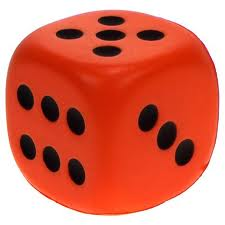
\includegraphics[width=.3\textwidth]{les04-dobbelsteen}
  \end{columns}
  
\end{frame}

\begin{frame}
  \frametitle{Kansverdeling voor één dobbelsteen}
  
  Wat is de kans om een aantal ogen te werpen met een dobbelsteen?
  
  \begin{center}
    \begin{tabular}{|c|c|c|c|c|c|}
      \hline
      1&2&3&4&5&6\\
      \hline
      \onslide<2->{$\frac{1}{6}}$ &\onslide<2->{$\frac{1}{6}}$ &\onslide<2->{$\frac{1}{6}}$ &\onslide<2->{$\frac{1}{6}}$ &\onslide<2->{$\frac{1}{6}}$ &     \onslide<2->{$\frac{1}{6}}$ \\
      \hline
      
    \end{tabular}
  \end{center}
  
  \onslide<2->{%
    \begin{center}
      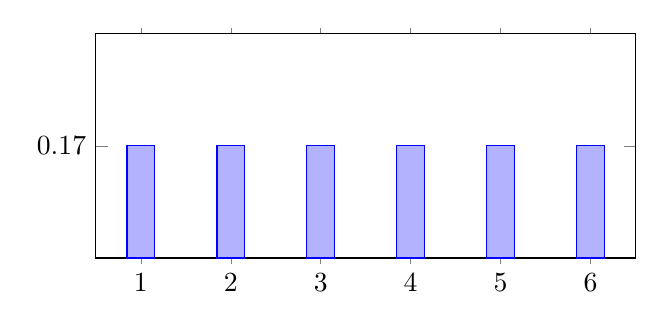
\begin{tikzpicture}
      \begin{axis}[ybar,ytick=data, anchor=north, yscale=.5]
      \addplot
      coordinates {
        (1, 1/6)
        (2, 1/6)
        (3, 1/6)
        (4, 1/6)
        (5, 1/6)
        (6, 1/6)};
      \end{axis}
      \end{tikzpicture}
  \end{center}}
  
\end{frame}

\begin{frame}
  \frametitle{Kansverdeling voor twee dobbelstenen}
  
  \begin{center}
    \begin{tabular}{|c|c|c|c|c|c|c|c|c|c|c|c|}
      \hline
      2&3&4&5&6&7&8&9&10&11&12\\
      \hline
      \onslide<2->{$\frac{1}{36}}$ &\onslide<2->{$\frac{2}{36}}$ &\onslide<2->{$\frac{3}{36}}$ &\onslide<2->{$\frac{4}{36}}$ &\onslide<2->{$\frac{5}{36}}$ & \onslide<2->{$\frac{6}{36}}$ & \onslide<2->{$\frac{5}{36}}$ &\onslide<2->{$\frac{4}{36}}$ & \onslide<2->{$\frac{3}{36}}$ &\onslide<2->{$\frac{2}{36}}$ &\onslide<2->{$\frac{1}{36}}$ \\
      \hline
      
    \end{tabular}
  \end{center}
  
  \onslide<2->{%
    \begin{center}
      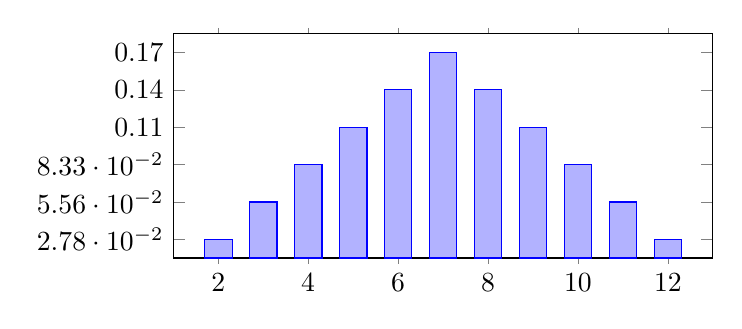
\begin{tikzpicture}
      \begin{axis}[ybar,ytick=data, anchor=north, yscale=.5]
      \addplot
      coordinates {
        (2, 1/36)
        (3, 2/36)
        (4, 3/36)
        (5, 4/36)
        (6, 5/36)
        (7, 6/36)
        (8, 5/36)
        (9, 4/36)
        (10, 3/36)
        (11, 2/36)
        (12, 1/36)
      };
      
      \end{axis}
      \end{tikzpicture}
    \end{center}
  }
  
\end{frame}

\pgfmathdeclarefunction{gauss}{2}{%
  \pgfmathparse{1/(#2*sqrt(2*pi))*exp(-((x-#1)^2)/(2*#2^2))}%
}

\begin{frame}
  \frametitle{Continue kansverdeling}
  
  De reactiesnelheid $x$ van Superman (in milliseconden) kun je als volgt weergegeven:
  
  \bigskip
  
  \begin{columns}
    \begin{column}{.85\textwidth}
      \begin{tikzpicture}
        \begin{axis}[
          domain=0:10, samples=100,
          axis lines*=left, xlabel=$x$ (ms), ylabel=$y$,
          every axis y label/.style={at=(current axis.above origin),anchor=south},
          every axis x label/.style={at=(current axis.right of origin),anchor=west},
          height=5cm, width=11cm,
          xtick={5,3.5,6.5}, ytick=\empty,
          enlargelimits=false, clip=false, axis on top,
          grid = major
          ]
          \addplot [fill=cyan!20, draw=none, domain=0:9] {gauss(5,1.5)} \closedcycle;
          \draw [yshift=-0.6cm, latex-latex](axis cs:3.5,0) -- node [fill=white] {$\sigma$} (axis cs:4.99,0);
          \draw [yshift=-0.6cm, latex-latex](axis cs:5.01,0) -- node [fill=white] {$\sigma$} (axis cs:6.5,0);
          \draw [-](axis cs:5,-0.035) -- (axis cs:5,-0.06);
          \node at (axis cs:5,-0.075) {$\mu$};
        \end{axis}
      \end{tikzpicture}
    \end{column}
    \begin{column}{.15\textwidth}
      
\includegraphics[width=1.5cm]{les2-hero-3}
    \end{column}
  \end{columns}
  
\end{frame}

\begin{frame}
  \frametitle{\textit{Standaard}normale verdeling}
  
  \begin{columns}[c]
    \column{.5\textwidth}
    normaalverdeling
    $x \in X \sim Nor(\mu, \sigma)$
    \begin{tikzpicture}
    \begin{axis}[
    domain=-2.5:2.5,
    axis lines*=left,
    xmin=-2.5, xmax=2.5,
    ymin=0, ymax=0.39,
    xlabel=$X$,
    every axis x label/.style={at=(current axis.right of origin),anchor=west},
    every axis y label/.style={at=(current axis.above origin),anchor=south},
    height=4cm, width=6cm,
    xtick={-1.4,0,1.4},
    xticklabels={$\mu-\sigma$,$\mu$,$\mu+\sigma$},
    ytick=\empty,
    enlargelimits=false,
    axis on top,
    clip=false,
    ]
    \addplot[very thick,smooth,draw=hgblue]{gauss(0,1.4)};
    \draw [-](axis cs:0.4,0) -- (axis cs:0.4,0.274); %vertical line
    \node at (axis cs: 0.56,0.1) {$x$}; %label x
    \draw [latex-latex](axis cs:2.2,0.22) -- (axis cs:3.5,0.22);
    \end{axis}
    \end{tikzpicture}
    \column{.5\textwidth}
    \textbf{standaard}normaalverdeling
    $z \in Z \sim Nor(0, 1)$
    \begin{tikzpicture}
    \begin{axis}[
    domain=-2.5:2.5,
    axis lines*=left,
    xmin=-2.5, xmax=2.5,
    ymin=0, ymax=0.39,
    xlabel=$Z$,
    every axis x label/.style={at=(current axis.right of origin),anchor=west},
    every axis y label/.style={at=(current axis.above origin),anchor=south},
    height=4cm, width=6cm,
    xtick={-1,0,1},
    enlargelimits=false,
    axis on top,
    clip=false,
    ]
    \addplot[very thick,smooth,draw=hgblue]{gauss(0,1)};
    \draw [-](axis cs:0.286,0) -- (axis cs:0.286,0.383); %vertical line
    \node at (axis cs: 0.42,0.12 ) {$z$}; %label z
    \end{axis}
    \end{tikzpicture}
  \end{columns}
  \vfill
  $x$ en $z$ hebben een vergelijkbare positie op de Gauss-curve.\\
  Wat is het wiskundig verband tussen $x$ en $z$?
  \vfill
  \pause
  {\Large $x = \mu + z . \sigma$} ~~~ and ~~~ {\Large $z = \frac{x - \mu}{\sigma}$}
\end{frame}

\begin{frame}
  \frametitle{Standaardnormale verdeling}
  
  % Bron: http://johncanning.net/wp/?p=1202
  \begin{center}
    \begin{tikzpicture}
    \begin{axis}[
    no markers, domain=0:10, samples=100,
    axis lines*=left,height=6cm, width=10cm,
    xtick={-3, -2, -1, 0, 1, 2, 3}, ytick=\empty,
    enlargelimits=false, clip=false, axis on top,
    grid = major
    ]
    \addplot [smooth,fill=cyan!20, draw=none, domain=-3:3] {gauss(0,1)} \closedcycle;
    \addplot [smooth,fill=orange!20, draw=none, domain=-3:-2] {gauss(0,1)} \closedcycle;
    \addplot [smooth,fill=orange!20, draw=none, domain=2:3] {gauss(0,1)} \closedcycle;
    \addplot [smooth,fill=blue!20, draw=none, domain=-2:-1] {gauss(0,1)} \closedcycle;
    \addplot [smooth,fill=blue!20, draw=none, domain=1:2] {gauss(0,1)} \closedcycle;
    \addplot[<->] coordinates {(-1,0.4) (1,0.4)};
    \addplot[<->] coordinates {(-2,0.3) (2,0.3)};
    \addplot[<->] coordinates {(-3,0.2) (3,0.2)};
    \node[coordinate, pin={68.3\%}] at (axis cs: 0, 0.35){};
    \node[coordinate, pin={95.4\%}] at (axis cs: 0, 0.25){};
    \node[coordinate, pin={99.7\%}] at (axis cs: 0, 0.15){};
    \node[coordinate, pin={34.1\%}] at (axis cs: -0.5, 0){};
    \node[coordinate, pin={34.1\%}] at (axis cs: 0.5, 0){};
    \node[coordinate, pin={13.6\%}] at (axis cs: 1.5, 0){};
    \node[coordinate, pin={13.6\%}] at (axis cs: -1.5, 0){};
    \node[coordinate, pin={2.1\%}] at (axis cs: 2.5, 0){};
    \node[coordinate, pin={2.1\%}] at (axis cs: -2.5, 0){};
    \end{axis}
    \end{tikzpicture}
  \end{center}
\end{frame}

\begin{frame}[fragile]
  \frametitle{Belangrijkste functies in R}
  
  Voor een normale verdeling met gemiddelde \texttt{m} en standaardafwijking \texttt{s}:
  \vfill
  \centering
  \begin{tabular}{ll}
    \textbf{Functie}      & \textbf{Betekenis}                          \\ \hline
    \verb|pnorm(x, m, s)| & Linkerstaartkans, $P(X<\mathtt{x})$         \\
    \verb|dnorm(x, m, s)| & Hoogte van de Gausscurve op punt \texttt{x} \\
    \verb|qnorm(p, m, s)| & Onder welke grens zal \texttt{p}\% van de   \\
    & waarnemingen liggen?                        \\
    \verb|rnorm(n, m, s)| & Genereer \texttt{n} normaal verdeelde random getallen
  \end{tabular}
  \vfill
  Argumenten \texttt{m} en \texttt{s} weglaten geeft waarden voor de \textit{\textbf{standaard}}normaalverdeling: \texttt{pnorm(x)=pnorm(x,0,1)}
\end{frame}

\begin{frame}
  \frametitle{Kansen berekenen}
  Hoe groot is de kans dat\dots\\
  \dots de reactiesnelheid van Superman meer dan 6 milliseconden is?
  \vfill
  Wiskundige notatie:\\
  \hspace{1cm}$P( X > 6)$ = ?\hspace{1cm}met $X \sim Nor(\mu=5,\sigma=1,5)$
  \vfill
  \begin{center}
    \begin{tikzpicture}
    \begin{axis}[
    domain=0:10,
    axis lines*=left,
    xlabel=$x$,
    every axis x label/.style={at=(current axis.right of origin),anchor=west},
    every axis y label/.style={at=(current axis.above origin),anchor=south},
    height=5cm, width=8cm,
    xtick={3.5,5,6.5},
    ytick=\empty,
    enlargelimits=false,
    axis on top,
    clip=false,
    ]
    \addplot[fill=cyan!20, draw=black, domain=6:10] {gauss(5,1.5)} \closedcycle;
    \addplot[very thick,smooth,draw=hgblue]{gauss(5,1.5)};
    \draw [-latex](axis cs:7,0.05) -- (axis cs:8.5,0.1);
    \node at (axis cs: 10, 0.1) {$P(X>6)$};
    \draw [-](axis cs:6,-0.005) -- (axis cs:6,-0.040);
    \node at (axis cs: 6, -0.055) {$6$};
    \end{axis}
    \end{tikzpicture}
  \end{center}
\end{frame}

\begin{frame}
  \frametitle{Kansen berekenen: $z$-tabel}
  
  $P( X > 6)$ = ?\hspace{1cm}met $X \sim Nor(\mu=5,\sigma=1,5)$
  
  \bigskip
  
  (Oude) berekeningsmethode met z-tabel, vb.
  
  \url{http://sixsigmastudyguide.com/wp-content/uploads/2014/04/z-table.jpg}
  
  \begin{enumerate}
    \pause
    \item zet om naar $z$-score\\
    $z=\frac{6-5}{1,5}=0,667$ dus $P(X>6) = P(Z>0,667)$
    \item zet eerst om naar een \textbf{\textit{linker}}staartkans
    \begin{itemize}
      \item regel van 100\% kans: $P(Z>0,667)=1-P(Z<0,667)$
      \item of symmetrie-regel: $P(Z>0,667)=P(Z<-0,667)$
    \end{itemize}
    \item zoek op in $z$-tabel\\
  \end{enumerate}
\end{frame}

\begin{frame}
  \frametitle{Kansen berekenen: met R}
  
  $P( X > 6)$ = ?\hspace{1cm}met $X \sim Nor(\mu=5,\sigma=1,5)$
  
  Rechtstreekse berekening met R (of rekenmachine)
  
  \begin{itemize}
    \pause
    \item zet eerst om naar een \textbf{\textit{linker}}staartkans:\\
    met regel van 100\% kans: $P(X>6)=1-P(X<6)$
    \item bereken met R: $1-P(X<6)=$\texttt{1-pnorm(6,5,1.5)}
  \end{itemize}
\end{frame}

\begin{frame}
  \frametitle{Voorbeelden}
  
  \begin{enumerate}
    \item Hoe groot is de kans dat de reactiesnelheid van Superman minder dan 4 ms is?
    \item Hoe groot is de kans dat hij in minder dan 7 ms reageert?
    \item Hoe groot is de kans dat Superman in minder dan 3 ms reageert?
    \item Hoe groot is de kans dat hij reageert tussen de 2 en de 6,5 ms?
    \item Binnen welke tijd ligt 80\% van zijn reactiesnelheid?
  \end{enumerate}
\end{frame}

\begin{frame}
  \frametitle{Vraag 3: $P(X<3)$}
  
  \begin{center}
    \begin{tikzpicture}
    \begin{axis}[no markers,domain=-4:4,axis lines*=left,yscale=.7,enlargelimits=false,clip=false]
    \addplot[very thick,smooth,draw=hgblue]{gauss(0, 1)};
    \addplot[smooth,fill=black!20, draw=black, domain=-4:-4/3] {gauss(0,1)} \closedcycle;
    
    \node at (axis cs: -1.33, -.05) {\small -1.33};
    \end{axis}
    \end{tikzpicture}
  \end{center}
\end{frame}

\begin{frame}
  \frametitle{Vraag 4: $P(2<X<6,5)$}
  
  \begin{center}
    \begin{tikzpicture}
    \begin{axis}[no markers,domain=-4:4,axis lines*=left,yscale=.7,enlargelimits=false,clip=false]
    \addplot[very thick,smooth,draw=hgblue]{gauss(0, 1)};
    \addplot[smooth,fill=black!20, draw=black, domain=-2:1] {gauss(0,1)} \closedcycle;
    
    \node at (axis cs: 1, -.05) {\small 1};
    \end{axis}
    \end{tikzpicture}
  \end{center}
\end{frame}

\begin{frame}
  \frametitle{Vraag 5}
  
  Voor welke $x$ is $P(X<x) = 80\%$?
  
  \vfill
  
  \begin{center}
    \begin{tikzpicture}
    \begin{axis}[no markers,domain=-4:4,axis lines*=left,yscale=.7,enlargelimits=false,clip=false]
    \addplot[very thick,smooth,draw=hgblue]{gauss(0, 1)};
    \addplot[smooth,fill=black!20, draw=black, domain=-4:.84] {gauss(0,1)} \closedcycle;
    
    \node at (axis cs: .84, -.05) {\small .84};
    \end{axis}
    \end{tikzpicture}
  \end{center}
\end{frame}

\section{De Centrale Limietstelling}

\begin{frame}
  \frametitle{De centrale limietstelling}
  
  \alertbox{Als de steekproefomvang voldoende groot is, dan kan de kansverdeling van het steekproefgemiddelde benaderd worden met een normale verdeling. Dit geldt ongeacht de vorm van de kansverdeling van de onderliggende populatie}
  
  \vfill
  
  \begin{columns}[c]
    \column{.33\textwidth}
    
\includegraphics[width=2cm]{les4-centrlimiet}
    \column{.33\textwidth}
    \begin{itemize}
      \item 1 test
      \item 25 tests
      \item 100 tests
    \end{itemize}
    \column{.33\textwidth}
    
\includegraphics[width=2cm]{les2-hero-3}
  \end{columns}
  
  \vfill
  Demo: \url{https://students.brown.edu/seeing-theory/probability-distributions/index.html}
\end{frame}

\begin{frame}
  \frametitle{De centrale limietstelling}
  Beschouw een aselecte steekproef van $n$ waarnemingen die uit een populatie met een willekeurige distributie met verwachtingswaarde $\mu$ en standaardafwijking $\sigma$. Als $n$ groot genoeg is zal de kansverdeling van $\overline{x}$ een normale verdeling benaderen met gemiddelde $\mu_{\overline{x}} = \mu$ en standaardafwijking $\sigma_{\overline{x}} = \frac{\sigma}{\sqrt{n}}$.
  
  \vspace{0.4cm}
  Hoe groter de steekproef is, des te beter zal de kansverdeling van $\overline{x}$ overeenkomen met een normaalverdeling.
\end{frame}

\section{Van steekproef naar populatie}

\begin{frame}
  \frametitle{Puntschatter}
  \alertbox{Een \textcolor{hgyellow}{puntschatter} voor een populatieparameter is een regel of een formule die ons zegt hoe we uit de steekproef een getal moeten berekenen om de populatieparameter te schatten.}
\end{frame}

\subsection{Betrouwbaarheidsintervallen}
\begin{frame}
  \frametitle{Betrouwbaarheidsinterval}
  \alertbox{Een \textcolor{hgyellow}{betrouwbaarheidsinterval} is een regel of een formule die ons zegt hoe we uit de steekproef een interval kunnen berekenen dat de waarde van de parameter met een zeker \textcolor{hgyellow}{betrouwbaarheidsniveau} bevat.}
\end{frame}

\subsection{Betrouwbaarheidsinterval grote steekproef}


\begin{frame}
  \frametitle{Grote steekproef}
  
  Gegeven een steekproef met gemiddelde $\overline{x}$.\\
  We zoeken nu een interval $\left[ ~\overline{x}-b~,~\overline{x}+b~\right]$ waarvan we met een betrouwbaarheidsniveau $(1-\alpha)$ van bvb. 95\% kunnen zeggen dat $\mu$ erbinnen ligt.
  \vfill
  \[ P\left( \overline{x}-b < \mu < \overline{x}+b \right) = 1-\alpha = 0,95 \]
  \vfill
  \begin{center}
    \begin{tikzpicture}[scale=.8]
    \begin{axis}[
    domain=-3:3,
    axis lines*=left,
    height=5cm, width=12cm,
    xtick={-1.96,0,1.96},
    xticklabels={$\overline{x}-b$,$\overline{x}$,$\overline{x}+b$},
    ytick=\empty,
    enlargelimits=false,
    axis on top,
    clip=false,
    ]
    \addplot[fill=cyan!20, draw=black, domain=-1.96:1.96] {gauss(0,1)} \closedcycle;
    \addplot[very thick,smooth,draw=hgblue]{gauss(0,1)};
    %\addplot[smooth,dashed,draw=hgblue]{gauss(0.8,1)};
    \node [text width=1.5cm,fill=cyan!20,align=center] at (axis cs: 0, 0.17) {95\%\\($1-\alpha$)};
    \draw [-latex](axis cs:2.15,0.02) -- (axis cs:2.4,0.07);
    \node [text width=1cm,fill=white,align=center] at (axis cs: 2.5,0.14) {2,5\%\\($\frac{\alpha}{2}$)};
    \draw [-latex](axis cs:-2.15,0.02) -- (axis cs:-2.3,0.07);
    \node [text width=1cm,align=center] at (axis cs: -2.3,0.14) {2,5\%\\($\frac{\alpha}{2}$)};
    \draw [-](axis cs:0.6,0.02) -- (axis cs:0.6,-0.06);
    \node [align=center] at (axis cs: 0.6,-0.09) {$\mu$};
    \end{axis}
    \end{tikzpicture}
  \end{center}
\end{frame}

\begin{frame}
  \frametitle{Grote steekproef}
  
  Dankzij de centrale limietstelling weten we dat
  $\overline{x} \in \overline{X} \sim Nor(\mu,\frac{\sigma}{\sqrt{n}})$
  
  En omwille van de symmetrie weten we dat
  \[ P\left( \overline{x}-b < \mu < \overline{x}-b \right) = P\left( \mu-b < \overline{x} < \mu+b \right) \]
  
  \vfill
  
  \begin{center}
    \begin{tikzpicture}[scale=.8]
    
    \begin{axis}[
    domain=-3:3,
    axis lines*=left,
    height=5cm, width=12cm,
    xlabel=$\overline{X}$,
    every axis x label/.style={at=(current axis.right of origin),anchor=west},
    every axis y label/.style={at=(current axis.above origin),anchor=south},
    xtick={-1.36,-0.4,0.6,1.6,2.56},
    xticklabels={$\mu-b$,,$\mu$,,$\mu+b$},
    ytick=\empty,
    enlargelimits=false,
    axis on top,
    clip=false,
    ]
    \addplot[fill=cyan!20, draw=black, domain=-1.36:2.56] {gauss(0.6,1)} \closedcycle;
    \addplot[very thick,smooth,draw=hgblue]{gauss(0.6,1)};
    \addplot[smooth,dashed,draw=hgblue]{gauss(0,1)};
    \node [text width=1.5cm,align=center] at (axis cs: 0.6, 0.17) {95\%\\($1-\alpha$)};
    \draw [-latex](axis cs:2.75,0.02) -- (axis cs:3.0,0.07);
    \node [text width=1cm,fill=white,align=center] at (axis cs: 3.1,0.14) {2,5\%\\($\frac{\alpha}{2}$)};
    \draw [-latex](axis cs:-1.55,0.02) -- (axis cs:-1.7,0.07);
    \node [text width=0.8cm,fill=white,align=center] at (axis cs: -1.8,0.14) {2,5\%\\($\frac{\alpha}{2}$)};
    \draw [-,dashed](axis cs:0,0.4) -- (axis cs:0,-0.07);
    \node [align=center] at (axis cs: 0,-0.1) {$\overline{x}$};
    \draw [latex-latex](axis cs:0.6,-0.07) -- node [fill=white] {$\frac{\sigma}{\sqrt{n}}$} (axis cs:1.6,-0.07);
    \end{axis}
    \end{tikzpicture}
  \end{center}
  
\end{frame}

\begin{frame}
  \frametitle{Grote steekproef}
  
  \bigskip
  
  We bepalen nu de $z$-score voor $\overline{x}$:
  $z = \frac{\overline{x} - \mu}{\frac{\sigma}{\sqrt{n}}}$
  
  We zoeken (in een tabel of rekentoestel) de waarde $z_\frac{\alpha}{2}$ waarbij:
  \[ P\left(-z_{\frac{\alpha}{2}} < z < z_{\frac{\alpha}{2}}\right) = 1 - \alpha = 0.95 \]
  \[ P\left(z < z_{\frac{\alpha}{2}}\right) = 1 - \frac{\alpha}{2} = 0.975 \]
  \[ z_{\frac{\alpha}{2}} = \texttt{qnorm(0.975)} \approx 1.96 \]
  
  \vfill
  
  
  \begin{center}
    \begin{tikzpicture}[scale=.8]
    \begin{axis}[
    domain=-3:3,
    axis lines*=left,
    xlabel=$Z$,
    every axis x label/.style={at=(current axis.right of origin),anchor=west},
    every axis y label/.style={at=(current axis.above origin),anchor=south},
    height=4cm, width=10cm,
    xtick={-1.96,-1,0,1,1.96},
    xticklabels={-$z_\frac{\alpha}{2}$,-1,0,1,$z_\frac{\alpha}{2}$},
    ytick=\empty,
    enlargelimits=false,
    axis on top,
    clip=false,
    ]
    \addplot[fill=cyan!20, draw=black, domain=-1.96:1.96] {gauss(0,1)} \closedcycle;
    \addplot[very thick,smooth,draw=hgblue]{gauss(0,1)};
    \node [text width=1.5cm,align=center] at (axis cs: 0, 0.15) {95\%\\($1-\alpha$)};
    \draw [-latex](axis cs:2.15,0.02) -- (axis cs:2.4,0.07);
    \node [text width=1cm,align=center] at (axis cs: 2.5,0.16) {2,5\%\\($\frac{\alpha}{2}$)};
    \draw [-latex](axis cs:-2.15,0.02) -- (axis cs:-2.3,0.07);
    \node [text width=1cm,align=center] at (axis cs: -2.3,0.16) {2,5\%\\($\frac{\alpha}{2}$)};
    
    \end{axis}
    \end{tikzpicture}
  \end{center}
  
\end{frame}

\begin{frame}
  \frametitle{Grote steekproef}
  
  We krijgen nu:
  \[ P\left(-1,96 < \frac{\overline{x} - \mu}{\frac{\sigma}{\sqrt{n}}} < 1,96 \right) = 0,95 \]
  \[ P\left( \mu-1,96 \frac{\sigma}{\sqrt{n}} < \overline{x} < \mu+1,96 \frac{\sigma}{\sqrt{n}} \right)  = 0,95 \]
  
  Wegens symmetrie kunnnen we $\mu$ en $\overline{x}$ verwisselen:
  \[ P\left( \overline{x}-1,96 \frac{\sigma}{\sqrt{n}} < \mu < \overline{x}+1,96 \frac{\sigma}{\sqrt{n}} \right)  = 0,95 \]
  
  We kunnen nu met 95\% zekerheid zeggen dat:
  \[ \mu \in \left[~\overline{x}-1,96.\frac{\sigma}{\sqrt{n}}~,~\overline{x}+1,96. \frac{\sigma}{\sqrt{n}}~\right] \]
  
  \small (in de praktijk gebruiken we $s_{steekpr}$ als schatting voor $\sigma_{populatie}$)
  
\end{frame}

\subsection{Kleine steekproef}
\begin{frame}
  \frametitle{Kleine steekproef}
  Bij een \textit{\textbf{kleine}} steekproef $(n < 30)$ is de centrale limietstelling \textbf{niet} meer geldig.
  \vfill
  Er geldt wél:\\
  \vfill
  Als een populatie $X$ normaal verdeeld is $(X \sim Nor(\mu,\sigma))$
  en je neemt een \textit{kleine} steekproef met gemiddelde $\overline{x}$ en standaardafwijking $s$,
  dan is
  \[ t = \frac{\overline{x} - \mu}{\frac{s}{\sqrt{n}}} \]
  verdeeld volgens een t-verdeling met ~$n-1$~ vrijheidsgraden\\
  (degrees of freedom)
  
\end{frame}

\begin{frame}
  \frametitle{De Student $t$-verdeling}
  \bigskip
  \centering
  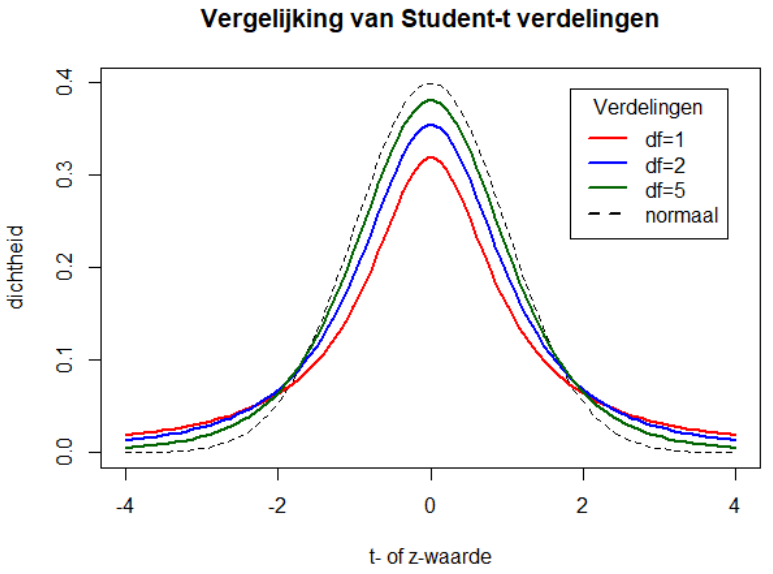
\includegraphics[height=.9\textheight]{les04-t-distrib}
\end{frame}

\begin{frame}
  \frametitle{Student $t$-verdeling in R}
  
  Voor een $t$-verdeling met ~\texttt{df}~ vrijheidsgraden:
  
  \small (\texttt{df = degrees of freedom})
  \vfill
  \centering
  \begin{tabular}{ll}
    \textbf{Functie}   & \textbf{Betekenis}                                         \\
    \hline
    \texttt{pt(x, df)} & Linkerstaartkans, $P(X<\mathtt{x})$                        \\
    \texttt{dt(x, df)} & Hoogte van de curve op punt \texttt{x}                     \\
    \texttt{qt(p, df)} & Onder welke grens zal \texttt{p}\% van de waarnemingen     \\
    & liggen?                                                    \\
    \texttt{rt(n, df)} & Genereer \texttt{n} random getallen volgens deze verdeling
  \end{tabular}
  
\end{frame}

\begin{frame}
  \frametitle{Betrouwbaarheidsinterval voor \textit{kleine} steekproef}
  Om een betrouwbaarheidsinterval voor het gemiddelde $\mu$ van een populatie te bepalen op basis van een \textit{kleine} steekproef, zoeken we eerst $t_ {\frac{\alpha}{2},df}$.
  
  \vfill
  Bij een betrouwbaarheidsniveau van 95\% is $\frac{\alpha}{2}=0,025$\\
  Veronderstel $n=5$ (dus \texttt{df=4}), dan is
  \[ t_ {\frac{\alpha}{2},df} = \texttt{qt(0.975,4)} = 2.776 \]
  
  \vfill
  We kunnen dan met 95\% zekerheid zeggen dat:
  \[ \mu \in \left[~ \overline{x} - t_{\frac{\alpha}{2},df}.\frac{s}{\sqrt{n}} ~,~ \overline{x} + t_{\frac{\alpha}{2},df}.\frac{s}{\sqrt{n}} ~\right] \]
  
\end{frame}


\subsection{Betrouwbaarheidsinterval voor fractie}
\begin{frame}
  \frametitle{Betrouwbaarheidsinterval voor fractie}
  \[ \overline{p} = \frac{\textnormal{aantal successen}}{n} \]
  \begin{itemize}
    \item Verwachting van kansverdeling van $\overline{p}$ is $p$.
    \item De standaardafwijking van kansverdeling $\overline{p}$ is $\sqrt{\frac{pq}{n}}$
    \item Voor grote steekproeven is $\overline{p}$ bij benadering normaal verdeeld.
  \end{itemize}
  Aangezien $\overline{p}$ een steekproefgemiddelde is van het aantal successen, stelt dit ons in staat een betrouwbaarheidsinterval te berekenen analoog als die voor de intervalschatting van $\mu$ voor grote steekproeven.
  
  
  \[ \overline{p} \pm z_{\frac{\alpha}{2}}.\sqrt{\frac{\overline{p}\overline{q}}{n}} \]
  met $\overline{p} = \frac{x}{n}$ en $\overline{q} = 1- \overline{p}$
  
\end{frame}


\end{document}